\documentclass[a4paper]{article}

%% Language and font encodings
\usepackage{polski}
\usepackage[polish]{babel}
\usepackage[utf8x]{inputenc}
\usepackage[T1]{fontenc}
\usepackage{pdfpages}
\usepackage{indentfirst}
\usepackage{listings}

% Adjust penalties
\brokenpenalty=1000
\clubpenalty=1000
\widowpenalty=1000

%% Sets page size and margins
\usepackage[a4paper]{geometry}

%% Useful packages
\usepackage{amsmath}
\usepackage{graphicx}
\usepackage[colorlinks=true, allcolors=blue]{hyperref}
\usepackage{booktabs}
\usepackage{cancel}
\usepackage{tikz}

\usepackage{float}

\renewcommand\thesection{\arabic{section}.}
\renewcommand\thesubsection{\arabic{section}.\arabic{subsection}.}
\renewcommand\thesubsubsection{\arabic{section}.\arabic{subsection}.\arabic{subsubsection}.}

% The following commands are not supported in PSTricks at present
% We define them conditionally, so when they are implemented,
% this pgf file will use them.
\ifx\du\undefined
  \newlength{\du}
\fi
\setlength{\du}{15\unitlength}

\newcommand{\Vsp}[1]{\vtop to #1 {}}
\newcommand{\Hsp}[1]{\hbox to #1 {}}
\newcommand{\Small}{\scriptsize}

\title{Sprawozdanie nr 1}
\date{}

\begin{document}

\begin{center}
\begin{tabular}{|p{5cm}|l|l|l|}
    \hline
    Wydział \Vsp{5mm} & \multicolumn{1}{|l}{Dzień} &  & Nr zespołu\\
    & \multicolumn{1}{|l}{Data} &  & \\
    \hline 
    Nazwisko i Imię: & \Small Ocena z przygotowania  & \Small Ocena ze sprawozdania & \Small Ocena Końcowa \\
    1. & & &\\
    2. & & & \\
    3. & & & \\
    \hline
    \multicolumn{2}{|l|}{Prowadzący \Vsp{1cm}} & \multicolumn{2}{|l|}{Podpis prowadzącego} \\
    \hline
\end{tabular}
\end{center}

{\let\newpage\relax\maketitle}  % stolen from: https://tex.stackexchange.com/questions/86249/maketitle-text-before-title
\setcounter{secnumdepth}{2}
\setcounter{tocdepth}{2}

\section{Prawo Ohma}

\subsection{Opis ćwiczenia}

Celem ćwiczenia jest wyznaczenie rezystancji oporników $R_1$, $R_2$, $R_3$ oraz $R_4$.
Obwód złożony jest z szeregowo podłączonego amperomierza cyfrowego, równolegle podłączonego woltomierza analogowego, rezystora oraz z zasilacza.

\begin{table}[h]
\centering
\begin{tikzpicture}[even odd rule]
\pgftransformxscale{1.000000}
\pgftransformyscale{-1.000000}
\definecolor{dialinecolor}{rgb}{0.000000, 0.000000, 0.000000}
\pgfsetstrokecolor{dialinecolor}
\pgfsetstrokeopacity{1.000000}
\definecolor{diafillcolor}{rgb}{1.000000, 1.000000, 1.000000}
\pgfsetfillcolor{diafillcolor}
\pgfsetfillopacity{1.000000}
\pgfsetlinewidth{0.100000\du}
\pgfsetdash{}{0pt}
\pgfsetbuttcap
\pgfsetmiterjoin
\pgfsetlinewidth{0.100000\du}
\pgfsetbuttcap
\pgfsetmiterjoin
\pgfsetdash{}{0pt}
\definecolor{dialinecolor}{rgb}{0.000000, 0.000000, 0.000000}
\pgfsetstrokecolor{dialinecolor}
\pgfsetstrokeopacity{1.000000}
\draw (14.654281\du,8.399077\du)--(17.279281\du,8.399077\du);
\pgfsetbuttcap
\pgfsetmiterjoin
\pgfsetdash{}{0pt}
{\pgfsetcornersarced{\pgfpoint{0.000000\du}{0.000000\du}}\definecolor{diafillcolor}{rgb}{1.000000, 1.000000, 1.000000}
\pgfsetfillcolor{diafillcolor}
\pgfsetfillopacity{1.000000}
\fill (17.279281\du,6.924077\du)--(17.279281\du,9.874077\du)--(22.529281\du,9.874077\du)--(22.529281\du,6.924077\du)--cycle;
}{\pgfsetcornersarced{\pgfpoint{0.000000\du}{0.000000\du}}\definecolor{dialinecolor}{rgb}{0.000000, 0.000000, 0.000000}
\pgfsetstrokecolor{dialinecolor}
\pgfsetstrokeopacity{1.000000}
\draw (17.279281\du,6.924077\du)--(17.279281\du,9.874077\du)--(22.529281\du,9.874077\du)--(22.529281\du,6.924077\du)--cycle;
}\pgfsetbuttcap
\pgfsetmiterjoin
\pgfsetdash{}{0pt}
\definecolor{dialinecolor}{rgb}{0.000000, 0.000000, 0.000000}
\pgfsetstrokecolor{dialinecolor}
\pgfsetstrokeopacity{1.000000}
\draw (22.529281\du,8.399077\du)--(25.154281\du,8.399077\du);
\pgfsetlinewidth{0.100000\du}
\pgfsetdash{}{0pt}
\pgfsetbuttcap
\pgfsetmiterjoin
\pgfsetlinewidth{0.100000\du}
\pgfsetbuttcap
\pgfsetmiterjoin
\pgfsetdash{}{0pt}
\definecolor{dialinecolor}{rgb}{0.000000, 0.000000, 0.000000}
\pgfsetstrokecolor{dialinecolor}
\pgfsetstrokeopacity{1.000000}
\draw (9.525000\du,12.450000\du)--(9.525000\du,13.887500\du);
\pgfsetbuttcap
\pgfsetmiterjoin
\pgfsetdash{}{0pt}
\definecolor{dialinecolor}{rgb}{0.000000, 0.000000, 0.000000}
\pgfsetstrokecolor{dialinecolor}
\pgfsetstrokeopacity{1.000000}
\draw (8.050000\du,13.887500\du)--(11.000000\du,13.887500\du);
\pgfsetbuttcap
\pgfsetmiterjoin
\pgfsetdash{}{0pt}
\definecolor{dialinecolor}{rgb}{0.000000, 0.000000, 0.000000}
\pgfsetstrokecolor{dialinecolor}
\pgfsetstrokeopacity{1.000000}
\draw (8.787500\du,14.462500\du)--(10.262500\du,14.462500\du);
\pgfsetbuttcap
\pgfsetmiterjoin
\pgfsetdash{}{0pt}
\definecolor{dialinecolor}{rgb}{0.000000, 0.000000, 0.000000}
\pgfsetstrokecolor{dialinecolor}
\pgfsetstrokeopacity{1.000000}
\draw (10.262500\du,13.025000\du)--(10.262500\du,13.600000\du);
\pgfsetbuttcap
\pgfsetmiterjoin
\pgfsetdash{}{0pt}
\definecolor{dialinecolor}{rgb}{0.000000, 0.000000, 0.000000}
\pgfsetstrokecolor{dialinecolor}
\pgfsetstrokeopacity{1.000000}
\draw (9.893750\du,13.312500\du)--(10.631250\du,13.312500\du);
\pgfsetbuttcap
\pgfsetmiterjoin
\pgfsetdash{}{0pt}
\definecolor{dialinecolor}{rgb}{0.000000, 0.000000, 0.000000}
\pgfsetstrokecolor{dialinecolor}
\pgfsetstrokeopacity{1.000000}
\draw (9.525000\du,14.462500\du)--(9.525000\du,15.900000\du);
\pgfsetlinewidth{0.100000\du}
\pgfsetdash{}{0pt}
\pgfsetbuttcap
\pgfsetmiterjoin
\pgfsetlinewidth{0.100000\du}
\pgfsetbuttcap
\pgfsetmiterjoin
\pgfsetdash{}{0pt}
\definecolor{diafillcolor}{rgb}{1.000000, 1.000000, 1.000000}
\pgfsetfillcolor{diafillcolor}
\pgfsetfillopacity{1.000000}
\pgfpathellipse{\pgfpoint{12.703705\du}{8.398236\du}}{\pgfpoint{1.105173\du}{0\du}}{\pgfpoint{0\du}{1.105173\du}}
\pgfusepath{fill}
\definecolor{dialinecolor}{rgb}{0.000000, 0.000000, 0.000000}
\pgfsetstrokecolor{dialinecolor}
\pgfsetstrokeopacity{1.000000}
\pgfpathellipse{\pgfpoint{12.703705\du}{8.398236\du}}{\pgfpoint{1.105173\du}{0\du}}{\pgfpoint{0\du}{1.105173\du}}
\pgfusepath{stroke}
\pgfsetbuttcap
\pgfsetmiterjoin
\pgfsetdash{}{0pt}
\definecolor{dialinecolor}{rgb}{0.000000, 0.000000, 0.000000}
\pgfsetstrokecolor{dialinecolor}
\pgfsetstrokeopacity{1.000000}
\draw (12.630026\du,7.735132\du)--(13.219452\du,8.913983\du);
\pgfsetbuttcap
\pgfsetmiterjoin
\pgfsetdash{}{0pt}
\definecolor{dialinecolor}{rgb}{0.000000, 0.000000, 0.000000}
\pgfsetstrokecolor{dialinecolor}
\pgfsetstrokeopacity{1.000000}
\draw (12.630026\du,7.735132\du)--(12.187957\du,8.913983\du);
\pgfsetbuttcap
\pgfsetmiterjoin
\pgfsetdash{}{0pt}
\definecolor{dialinecolor}{rgb}{0.000000, 0.000000, 0.000000}
\pgfsetstrokecolor{dialinecolor}
\pgfsetstrokeopacity{1.000000}
\draw (12.408992\du,8.324558\du)--(12.924739\du,8.324558\du);
\pgfsetbuttcap
\pgfsetmiterjoin
\pgfsetdash{}{0pt}
\definecolor{dialinecolor}{rgb}{0.000000, 0.000000, 0.000000}
\pgfsetstrokecolor{dialinecolor}
\pgfsetstrokeopacity{1.000000}
\draw (10.346003\du,8.398236\du)--(11.598532\du,8.398236\du);
\pgfsetbuttcap
\pgfsetmiterjoin
\pgfsetdash{}{0pt}
\definecolor{dialinecolor}{rgb}{0.000000, 0.000000, 0.000000}
\pgfsetstrokecolor{dialinecolor}
\pgfsetstrokeopacity{1.000000}
\draw (13.808877\du,8.398236\du)--(15.061406\du,8.398236\du);
\pgfsetlinewidth{0.100000\du}
\pgfsetdash{}{0pt}
\pgfsetbuttcap
{
\definecolor{diafillcolor}{rgb}{0.000000, 0.000000, 0.000000}
\pgfsetfillcolor{diafillcolor}
\pgfsetfillopacity{1.000000}
% was here!!!
\definecolor{dialinecolor}{rgb}{0.000000, 0.000000, 0.000000}
\pgfsetstrokecolor{dialinecolor}
\pgfsetstrokeopacity{1.000000}
\draw (15.061406\du,8.398236\du)--(14.654281\du,8.399077\du);
}
\pgfsetlinewidth{0.100000\du}
\pgfsetdash{}{0pt}
\pgfsetmiterjoin
\pgfsetbuttcap
{
\definecolor{diafillcolor}{rgb}{0.000000, 0.000000, 0.000000}
\pgfsetfillcolor{diafillcolor}
\pgfsetfillopacity{1.000000}
% was here!!!
{\pgfsetcornersarced{\pgfpoint{0.000000\du}{0.000000\du}}\definecolor{dialinecolor}{rgb}{0.000000, 0.000000, 0.000000}
\pgfsetstrokecolor{dialinecolor}
\pgfsetstrokeopacity{1.000000}
\draw (10.346003\du,8.398236\du)--(10.346003\du,8.395940\du)--(9.525000\du,8.395940\du)--(9.525000\du,12.450000\du);
}}
\pgfsetlinewidth{0.100000\du}
\pgfsetdash{}{0pt}
\pgfsetbuttcap
\pgfsetmiterjoin
\pgfsetlinewidth{0.100000\du}
\pgfsetbuttcap
\pgfsetmiterjoin
\pgfsetdash{}{0pt}
\definecolor{diafillcolor}{rgb}{1.000000, 1.000000, 1.000000}
\pgfsetfillcolor{diafillcolor}
\pgfsetfillopacity{1.000000}
\pgfpathellipse{\pgfpoint{14.875098\du}{13.806110\du}}{\pgfpoint{1.049258\du}{0\du}}{\pgfpoint{0\du}{1.049258\du}}
\pgfusepath{fill}
\definecolor{dialinecolor}{rgb}{0.000000, 0.000000, 0.000000}
\pgfsetstrokecolor{dialinecolor}
\pgfsetstrokeopacity{1.000000}
\pgfpathellipse{\pgfpoint{14.875098\du}{13.806110\du}}{\pgfpoint{1.049258\du}{0\du}}{\pgfpoint{0\du}{1.049258\du}}
\pgfusepath{stroke}
\pgfsetbuttcap
\pgfsetmiterjoin
\pgfsetdash{}{0pt}
\definecolor{dialinecolor}{rgb}{0.000000, 0.000000, 0.000000}
\pgfsetstrokecolor{dialinecolor}
\pgfsetstrokeopacity{1.000000}
\draw (14.805148\du,14.295764\du)--(15.364752\du,13.176555\du);
\pgfsetbuttcap
\pgfsetmiterjoin
\pgfsetdash{}{0pt}
\definecolor{dialinecolor}{rgb}{0.000000, 0.000000, 0.000000}
\pgfsetstrokecolor{dialinecolor}
\pgfsetstrokeopacity{1.000000}
\draw (14.805148\du,14.295764\du)--(14.385444\du,13.176555\du);
\pgfsetbuttcap
\pgfsetmiterjoin
\pgfsetdash{}{0pt}
\definecolor{dialinecolor}{rgb}{0.000000, 0.000000, 0.000000}
\pgfsetstrokecolor{dialinecolor}
\pgfsetstrokeopacity{1.000000}
\draw (14.875098\du,11.637643\du)--(14.875098\du,12.756852\du);
\pgfsetbuttcap
\pgfsetmiterjoin
\pgfsetdash{}{0pt}
\definecolor{dialinecolor}{rgb}{0.000000, 0.000000, 0.000000}
\pgfsetstrokecolor{dialinecolor}
\pgfsetstrokeopacity{1.000000}
\draw (14.875098\du,14.855368\du)--(14.875098\du,16.044527\du);
\pgfsetlinewidth{0.100000\du}
\pgfsetdash{}{0pt}
\pgfsetbuttcap
{
\definecolor{diafillcolor}{rgb}{0.000000, 0.000000, 0.000000}
\pgfsetfillcolor{diafillcolor}
\pgfsetfillopacity{1.000000}
% was here!!!
\definecolor{dialinecolor}{rgb}{0.000000, 0.000000, 0.000000}
\pgfsetstrokecolor{dialinecolor}
\pgfsetstrokeopacity{1.000000}
\draw (14.857844\du,8.398656\du)--(14.875098\du,11.637643\du);
}
\pgfsetlinewidth{0.100000\du}
\pgfsetdash{}{0pt}
\pgfsetmiterjoin
\pgfsetbuttcap
{
\definecolor{diafillcolor}{rgb}{0.000000, 0.000000, 0.000000}
\pgfsetfillcolor{diafillcolor}
\pgfsetfillopacity{1.000000}
% was here!!!
{\pgfsetcornersarced{\pgfpoint{0.000000\du}{0.000000\du}}\definecolor{dialinecolor}{rgb}{0.000000, 0.000000, 0.000000}
\pgfsetstrokecolor{dialinecolor}
\pgfsetstrokeopacity{1.000000}
\draw (9.525000\du,15.900000\du)--(9.525000\du,15.994225\du)--(14.875098\du,15.994225\du)--(14.875098\du,16.044527\du);
}}
\pgfsetlinewidth{0.100000\du}
\pgfsetdash{}{0pt}
\pgfsetmiterjoin
\pgfsetbuttcap
{
\definecolor{diafillcolor}{rgb}{0.000000, 0.000000, 0.000000}
\pgfsetfillcolor{diafillcolor}
\pgfsetfillopacity{1.000000}
% was here!!!
{\pgfsetcornersarced{\pgfpoint{0.000000\du}{0.000000\du}}\definecolor{dialinecolor}{rgb}{0.000000, 0.000000, 0.000000}
\pgfsetstrokecolor{dialinecolor}
\pgfsetstrokeopacity{1.000000}
\draw (14.875098\du,16.029376\du)--(14.875098\du,15.992274\du)--(25.154281\du,15.992274\du)--(25.154281\du,8.409077\du);
}}
% setfont left to latex
\definecolor{dialinecolor}{rgb}{0.000000, 0.000000, 0.000000}
\pgfsetstrokecolor{dialinecolor}
\pgfsetstrokeopacity{1.000000}
\definecolor{diafillcolor}{rgb}{0.000000, 0.000000, 0.000000}
\pgfsetfillcolor{diafillcolor}
\pgfsetfillopacity{1.000000}
\node[anchor=base west,inner sep=0pt,outer sep=0pt,color=dialinecolor] at (19.404296\du,8.774988\du){\Huge \sffamily R};
\end{tikzpicture}

\caption{Schemat układu pomiarowego}
\end{table}

\subsection{Wstęp teoretyczny}

\subsubsection{Prawo Ohma}

Prądem nazywamy uporządkowany ruch ładunków elektrycznych.
W obwodzie elektrycznym stosunek napięcia do natężenia prądu jest stały:

$$\frac{U}{I} = \text{const}$$

Powyższa zależność jest nazywana \emph{prawem Ohma}. Współczynnik proporcjonalności nazywamy \emph{rezystancją} (oporem), mierzymy ją w omach ($\Omega$) i zwyczajowo oznaczamy za pomocą litery $R$.

\subsubsection{Niepewności pomiarowe}

Niepewnością pomiarową nazywamy miarę dokładności wykonanego pomiaru.
Wśród pomiarów bezpośrednich wyróżniamy dwa rodzaje metod wyliczania niepewności.

\begin{itemize}
\item Metody typu A -- jest to klasa metod, która oblicza niepewność za pomocą statystycznych technik analizy ciągu 	wyników pomiarów;
\item Metody typu B -- klasa metod, które opierają się na innych metod niż metody typu A, np.~metody biorące pod uwagę własności przyrządów pomiarowych.
\end{itemize}

\subsection{Analiza wyników}

Pierwsze ćwiczenie polegało na zbadaniu relacji między napięciem a natężeniem prądu.
W tym celu dokonaliśmy 10 pomiarów napięcia na rezystorze $R_4$ oraz 10 pomiarów natężenia prądu płynącego w obwodzie.
Uzyskane wyniki zostały przedstawione w tabeli (Rysunek \ref{wykres}) oraz na wykresie zależności napięcia na $R_4$ od natężenia prądu (Tablica \ref{pomiary_r4}).

\begin{figure}[h]
\centering
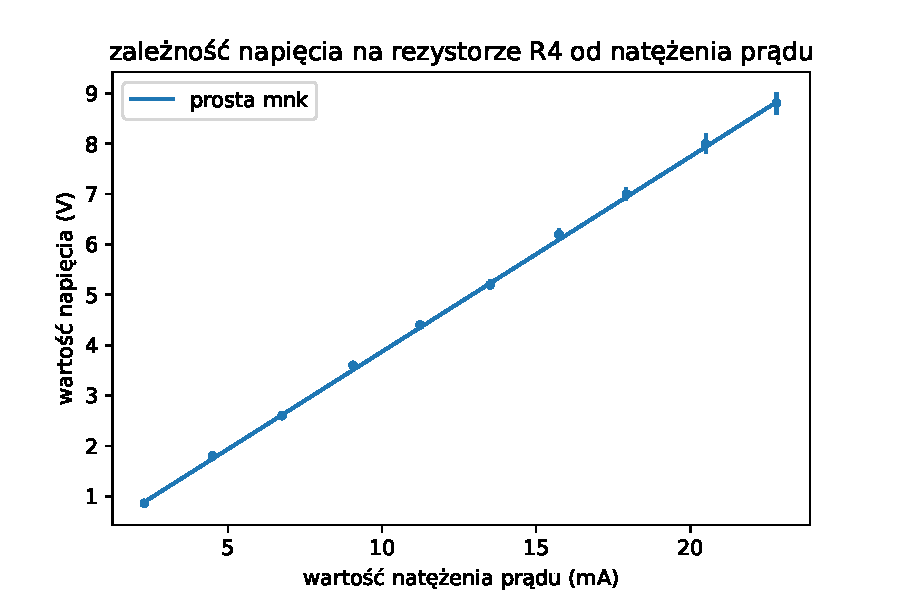
\includegraphics[scale=0.7]{fig_d.pdf}
\caption{Wyliczona prosta regresji liniowej zestawiona wraz ze zmierzonymi wartościami napięcia oraz natężenia prądu.}
\label{wykres}
\end{figure}

\newpage

Dla użytego woltomierza, przy zakresie $Z(U)$, niepewność wyznaczenia napięcia wynosi:

$$u_U = \frac{1\% \cdot Z(U)}{\sqrt{3}}$$

Niepewność wyznaczenia natężenia prądu (przy użytym amperomierzu) jest zależna od odczytanej wartości i wynosi:

$$u_I = \frac{1.2\% \text{rdg} + 1 \text{dgt}}{\sqrt{3}}$$

\begin{table}
\centering
\begin{tabular}{rrrrrrr}
\toprule
Lp. &  $U$ (V) &  $Z(U)$ (V) &  $u_U$ (V) &  $I$ (mA) &  $Z(I)$ (mA) &  $u_I$ (mA) \\
\midrule
1 &          8.800  &                10 &                 0.058  &             22.80  &                200 &                     0.22 \\
2 &          8.000  &                10 &                 0.058  &             20.50  &                200 &                     0.20 \\
3 &          7.000  &                10 &                 0.058  &             17.930 &                 20 &                     0.058 \\
4 &          6.200  &                10 &                 0.058  &             15.740 &                 20 &                     0.051 \\
5 &          5.200  &                10 &                 0.058  &             13.510 &                 20 &                     0.045 \\
6 &          4.400  &                10 &                 0.058  &             11.230 &                 20 &                     0.038 \\
7 &          3.600  &                10 &                 0.058  &              9.060 &                 20 &                     0.032 \\
8 &          2.600  &                 3 &                 0.017  &              6.760 &                 20 &                     0.025 \\
9 &          1.800  &                 3 &                 0.017  &              4.500 &                 20 &                     0.019 \\
10 &         0.8600 &                 1 &                 0.0058 &              2.290 &                 20 &                     0.012 \\
\bottomrule
\end{tabular}
\caption{Wielokrotne pomiary prądu $I_{R_4}$ i napięcia $U_{R_4}$ na rezystorze $R_4$.}
\label{pomiary_r4}
\end{table}

Na podstawie pomiarów napięcia i natężenia -- oraz uwzględniając błędy pomiarowe -- możemy stwierdzić, że natężenie prądu rośnie wprost proporcjonalnie do napięcia.
Stosunek napięcia do natężenia jest stały.
Wyniki doświadczenia potwierdzają słuszność prawa Ohma.

\subsection{Regresja liniowa}

Używając metody najmniejszych kwadratów można wyznaczyć współczynnik kierunkowy prostej $y = ax + b$.
Ponieważ napięcie i natężenie prądu są powiązane postacią $U = RI$, to przyjmujemy $b = 0$.
Zatem dopasowywana prosta będzie postaci $y = ax$.

Współczynnik kierunkowy szukanej prostej będzie szukaną rezystancją opornika. Ponadto, rezystancja ta będzie wyrażona wzorem:

$$R = a = \frac{\sum_{i = 1}^{10}\frac{I_i U_i}{u_{U_i}^2}}{\sum_{i = 1}^{10}\frac{I_i^2}{u_{U_i}^2}}$$

Z niepewnością wynoszącą:

$$u_a = \sqrt{\frac{1}{\sum_{i = 1}^{10}\frac{I_i^2}{u_{U_i}^2}}}$$

W celu wyznaczenia powyższych wartości pomocna będzie tabela z pośrednimi wartościami obliczeń (Tablica \ref{wartosci_posrednie}). Zachowano w niej dodatkowe cyfry znaczące, aby uniknąć błędów numerycznych przy kolejnych obliczeniach.


Otrzymujemy $a = \frac{313502.546}{805575.221} \approx 0.3892 \enskip \text{k} \Omega = 389.2 \enskip \Omega $ 

oraz $\enskip u_a = \sqrt{\frac{1}{805575.221}} \approx 0.0011 \enskip \text{k}\Omega = 1.1 \enskip \Omega$.

Zatem opór $R_4 = 389.2 \, (1.1) \enskip \Omega$.
\vspace{2em}

\begin{table}[h]
\centering
\begin{tabular}{lrrrrrrrrr}
\toprule
{} &  $U$  &    $u_U$  &     $I$ &    $u_I$   &    $IU$  &    $u_U^2$ &   $I^2$ &    $\frac{I^2}{u_U^2}$ & $\frac{IU}{u_U^2}$ \\
\midrule
1  &  8.80 &  0.0577350 &  22.80 &  0.215698  & 200.64   &  0.00333 &  519.84    & 155953.560  & 60192.602 \\
2  &  8.00 &  0.0577350 &  20.50 &  0.199763  & 164.00   &  0.00333 &  420.25    & 126076.261  & 49200.492 \\
3  &  7.00 &  0.0577350 &  17.93 &  0.057533  & 125.51   &  0.00333 &  321.4849  &  96446.434  & 37653.377 \\
4  &  6.20 &  0.0577350 &  15.74 &  0.051211  &  97.588  &  0.00333 &  247.7476  &  74325.023  & 29276.693 \\
5  &  5.20 &  0.0577350 &  13.51 &  0.044774  &  70.252  &  0.00333 &  182.5201  &  54756.578  & 21075.811 \\
6  &  4.40 &  0.0577350 &  11.23 &  0.038192  &  49.412  &  0.00333 &  126.1129  &  37834.248  & 14823.748 \\
7  &  3.60 &  0.0577350 &   9.06 &  0.031928  &  32.616  &  0.00333 &   82.0836  &  24625.326  &  9784.898 \\
8  &  2.60 &  0.0173205 &   6.76 &  0.025288  &  17.576  &  0.00030 &   45.6976  & 152325.333  & 58586.667 \\
9  &  1.80 &  0.0173205 &   4.50 &  0.018764  &   8.1    &  0.00030 &   20.25    &  67500.000  & 27000.000 \\
10 &  0.86 &  0.0057735 &   2.29 &  0.012384  &   1.9694 &  0.00003 &    5.2441  &  15732.457  &  5908.259 \\
\midrule
	suma & {} & {} & {} & {} & {} & {} & {} & 805575.221 & 313502.546 \\
\bottomrule
\end{tabular}
\caption{Wartości pośrednie obliczeń, które pozwalają wyznaczyć wartość współczynnika kierunkowego w zagadnieniu regresji liniowej}
\label{wartosci_posrednie}
\end{table}


\subsection{Obliczenia wartości $R_1$, $R_2$, $R_3$}

Wyniki pomiarów umieszczono w tablicy \ref{pomiary_r123}.

Niepewności napięcia oraz natężenia prądu są liczone jak wyżej.

Niepewność rezystancji wyznaczonej za pomocą wzoru $R = \frac{U}{I}$ wynosi:

$$u_R = \sqrt{(\frac{\partial R}{\partial U})^2 \cdot u_U^2 + (\frac{\partial R}{\partial I})^2 \cdot u_I^2} = \sqrt{\frac{1}{I^2} \cdot u_U + \frac{U^2}{I^2} \cdot u_I}$$



Zatem wartości $R_1$, $R_2$, $R_3$ wynoszą (zapis na trzy sposoby):

\begin{itemize}
\item $R_1 = 51.537 \enskip \Omega$, $u_{R_1} = 0.035 \enskip \Omega$

$R_2 = 103.90 \enskip \Omega$, $u_{R_2} = 0.06 \enskip \Omega$

$R_3 = 103.90 \enskip \Omega$, $u_{R_3} = 0.06 \enskip \Omega$

\item $R_1 = 51.537 \, (35) \enskip \Omega$

$R_2 = 103.90 \, (6) \enskip \Omega$

$R_3 = 103.90 \, (6) \enskip \Omega$

\item $R_1 = 51.537 \, (0.035) \enskip \Omega$

$R_2 = 103.90 \, (0.06) \enskip \Omega$

$R_3 = 103.90 \, (0.06) \enskip \Omega$
\end{itemize}

\begin{table}
\centering
\begin{tabular}{lrrrrrrl}
\toprule
Rezystor &  $U$ (V) &  $u_U$ (V) &  $I$ (mA) &  $u_I$ (mA) &  R ($\Omega$) &  $u_R$ ($\Omega$) \\
\midrule
$R_1$ &          2.85 &           0.018 &                  55.30 &              0.45 &             51.537 &             0.035 \\
$R_2$ &          4.0 &           0.06 &                  38.50 &              0.33 &            103.90 &             0.06 \\
$R_3$ &          4.0 &           0.06 &                  38.50 &              0.33 &            103.90 &             0.06 \\
\bottomrule
\end{tabular}
\caption{Wyniki pojedynczych pomiarów na rezystorach $R_1$, $R_2$ oraz $R_3$}
\label{pomiary_r123}
\end{table}


\newpage

\section{Pomiary wielkości mechanicznych}

\subsection{Opis ćwiczenia}
Celem ćwiczenia jest pomiar trzech wymiarów metalowej płytki oraz wyznaczenie jej objętości, wraz z niepewnościami.

\subsection{Pomiary za pomocą suwmiarki}

Przy użyciu suwmiarki dokonano dwukrotnego pomiaru długości ($l_1$, $l_2$) oraz jednokrotnego pomiaru szerokości ($l_3$).

Rozdzielczość suwmiarki wynosi $\Delta x = 0.02$ mm, zatem niepewność typu B wynosi: 

$u_B(x) = \frac{\Delta x}{\sqrt{3}} \approx 0.01154700 \approx 0.012$ mm.

Uzyskane pomiary w serii wyniosły kolejno: $36.600$ mm, $37.420$ mm, $30.700$ mm.

Zatem wartości $l_1$, $l_2$, $l_3$ wynoszą (zapis na trzy sposoby):


\begin{itemize}
\item $l_1 = 36.600 \enskip \text{mm}$, $u_B = 0.012 \enskip \text{mm}$

$l_2 = 37.420 \enskip \text{mm}$, $u_B = 0.012 \enskip \text{mm}$

$l_3 = 30.700 \enskip \text{mm}$, $u_B = 0.012 \enskip \text{mm}$

\item $l_1 = 36.600 \, (12) \enskip \text{mm}$

$l_2 = 37.420 \, (12) \enskip \text{mm}$ 

$l_3 = 30.700 \, (12) \enskip \text{mm}$

\item $l_1 = 36.600 \, (0.012) \enskip \text{mm}$

$l_2 = 37.420 \, (0.012) \enskip \text{mm}$

$l_3 = 30.700 \, (0.012) \enskip \text{mm}$
\end{itemize}

\subsection{Pomiary za pomocą śruby mikrometrycznej}

W tym ćwiczeniu, za pomocą śruby mikrometrycznej, badana była grubość metalowej płytki.
Wykonane pomiary ($n=60$) przedstawione zostały w tablicy \ref{pomiary_sruba} oraz za pomocą histogramu (tablica \ref{histogram_sruba}).

\textit{Uwaga}: pomiar wynoszący $2.97$ uznajemy za \textit{błąd gruby}.
W tabeli ten fakt został zaznaczony poprzez skreślenie, zaś w histogramie (oraz wszelkich obliczeniach) pomiar ten został pominięty.

\begin{table}[h]
\centering
\begin{tabular}{|l|l|l|l|l|l|}
\hline
2.94 & 2.93 & 2.94 & 2.92 & 2.94 & 2.95 \\
\hline
2.93 & 2.93 & \cancel{2.97} & 2.94 & 2.93 & 2.93 \\
\hline
2.93 & 2.94 & 2.93 & 2.93 & 2.94 & 2.93 \\
\hline
2.94 & 2.93 & 2.94 & 2.92 & 2.93 & 2.94 \\
\hline
2.93 & 2.94 & 2.94 & 2.93 & 2.94 & 2.94 \\
\hline
2.94 & 2.95 & 2.95 & 2.93 & 2.93 & 2.94 \\
\hline
2.94 & 2.93 & 2.94 & 2.94 & 2.94 & 2.93 \\
\hline
2.94 & 2.94 & 2.94 & 2.94 & 2.94 & 2.93 \\
\hline
2.94 & 2.93 & 2.93 & 2.94 & 2.93 & 2.94 \\
\hline
2.94 & 2.94 & 2.94 & 2.94 & 2.93 & 2.93 \\
\hline
\end{tabular}
\caption{Wyniki wielokrotnych pomiarów grubości płytki za pomocą śruby mikrometrycznej.}
\label{pomiary_sruba}
\end{table}

\begin{table}[h]
\centering
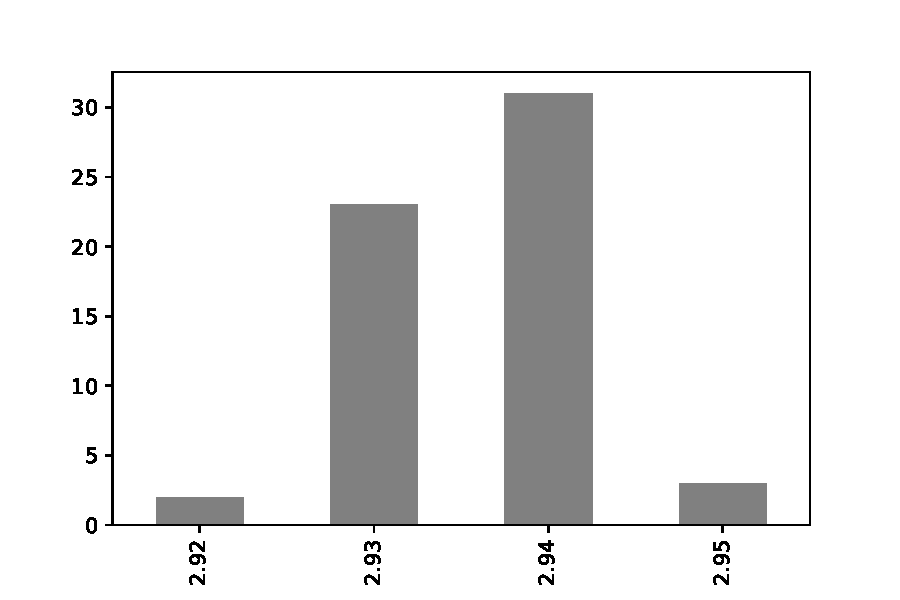
\includegraphics[scale=0.7]{hist.pdf}
\caption{Histogram pomiarów grubości płytki za pomocą śruby mikrometrycznej.}
\label{histogram_sruba}
\end{table}


Oznaczmy pomiary jako $x_i$, $i = 1, \dots, 59$.

Średnia wartość wszystkich pomiarów wynosi: $x = \frac{1}{59} \sum_{i = 1}^{59} x_i = \frac{1}{59} \cdot 173.22 \approx 2.935932203389$.

Odchylenie standardowe: $s_x = \sqrt{\frac{\sum_{i=1}^{59} (x_i - x)^2}{59 - 1}} \approx 0.0064643969$.

Niepewność typu A: $u_x (\text{typ A}) = \frac{s_x}{\sqrt{59}} \approx 0.00084159279 \enskip \text{mm} \approx 0.00084 \enskip \text{mm}$.

Niepewność typu B: $u_x (\text{typ B}) = \sqrt{\frac{(\Delta x)^2}{3} + \frac{(\Delta x_e)^2}{3}} = \sqrt{\frac{(0.01)^2}{3} + \frac{(0.005)^2}{3}} \approx 0.006454972 \approx 0.00645 \enskip \text{mm}$.

Niepewność całkowita: $u_x = \sqrt{(u_x (\text{typ A}))^2 + (u_x (\text{typ B}))^2} \approx 0.006504467695 \approx 0.0065 \enskip \text{mm}$.

Ostatecznie, grubość płytki wynosi (zapis na 3 sposoby):
\begin{itemize}
\item $d = 2.9365$ mm, $u_x = 0.0065$ mm
\item $d = 2.9365 \, (65)$ mm
\item $d = 2.9365 \, (0.0065)$ mm
\end{itemize}

\subsection{Wyznaczanie objętości płytki}

Zmierzone zostały trzy wymiary metalowej płytki.
Jako pierwszy wymiar ($x$) przyjmiemy średnią arytmetyczną dwóch pomiarów z niepewnością typu B.
Oznaczmy objętość $V = x \cdot y \cdot z$, gdzie $x = 37.510 \, (0.012)$ mm, $y = 30.700 \, (0.012)$ mm, $z = 2.9365 \, (0.0066)$ mm.
Zauważmy, że $x$ oraz $y$ są obarczone niepewnościami typu B, zaś $z$ niepewnością typu A oraz B.
W celu wyznaczenia objętości $V$ wraz z niepewnością całkowitą, posłużymy się następującymi oznaczeniami oraz wzorami:

$$V = x \cdot y \cdot z = 37.010 \cdot 30.700 \cdot 2.9365 \enskip \text{mm}^3 = 3336.4718555 \enskip \text{mm}^3 \approx 3336 \enskip \text{mm}^3$$

\begin{align*}
u_V &= \sqrt{(\frac{\partial V}{\partial x})^2 \cdot u_x^2 + (\frac{\partial V}{\partial y})^2 \cdot u_y^2 + (\frac{\partial V}{\partial z})^2 \cdot (u_z \text{(typ A)})^2 + (\frac{\partial V}{\partial z})^2 \cdot (u_z \text{(typ B)})^2} \\
	&= \sqrt{(yz \cdot u_x)^2 + (xz \cdot u_y)^2 + (xy \cdot u_z \text{(typ A)})^2 + (xy \cdot u_z \text{(typ B)})^2} \\
	&= \sqrt{(30.7 \cdot 2.9365 \cdot 0.012)^2 + (37.01 \cdot 2.9365 \cdot 0.012)^2 + (37.01 \cdot 30.7 \cdot 0.0009))^2 + (37.01 \cdot 30.7 \cdot 0.0065)^2} \enskip \text{mm}^3\\
	&\approx 58.4370490542980344 \enskip \text{mm}^3 \\
	&\approx 58 \enskip \text{mm}^3
\end{align*}

Ostatecznie, objętość płytki wynosi (zapis na 3 sposoby):

\begin{itemize}
\item $V = 3336 \enskip \text{mm}^3$, $u_V = 58 \enskip \text{mm}^3$
\item $V = 3336 \, (58) \enskip \text{mm}^3$
\item $V = 3336 \, (58) \enskip \text{mm}^3$
\end{itemize}

\end{document}
